\documentclass[acmsmall,screen,review,anonymous]{acmart}
\acmJournal{POMACS}
\settopmatter{printacmref=false}
\usepackage{booktabs}
\newcommand{\TV}{\mathrm{TV}}
\newcommand{\KL}{D_{\mathrm{KL}}}
\newcommand{\E}{\mathbb{E}}
\newcommand{\todo}[1]{}
\AtBeginDocument{\newtheorem{remark}[theorem]{Remark}}
\begin{document}
\title{The Value of Delayed Information: Predictive-Information Envelopes for Age-Limited Decisions}
\author{Anonymous Author(s)}
\begin{abstract}
A controller that acts on information of age $D$ --- a sensing delay, a
telemetry lag, a stale cache --- can outperform the best static policy only to
the extent that the delayed observation still \emph{predicts} the current
state. A companion systems submission \cite{infocom} proves this exactly for
symmetric two-state Markov capacity ($\Delta(D)=\tfrac12 r(D)$, the
autocorrelation at the sensing lag) with a $\beta$-mixing converse. This paper
supplies the general theory. We (i) isolate the exact object --- the
\emph{Bayes envelope} $\Delta_Y = \E[\psi(\mu_Y)]-\psi(\bar\mu)$, the expected
excess value of posterior over prior beliefs; (ii) restate, in
value-of-information form, the \emph{predictive-information envelope}
$0\le\Delta_Y\le\Omega\sqrt{\tfrac12 I(X;Y)}$ for bounded objectives with
oscillation $\Omega$ --- an inequality known in the minimum-excess-risk
literature, whose decision-value reading and operational inversion are
the contribution here --- together with its \emph{incremental} refinement --- the value of
a richer delayed observation over a coarser one is bounded by
$\Omega\sqrt{\tfrac12 I(X;H\mid Z)}$, so incremental decision value
certifies \emph{conditional} predictive information; (iii) derive the
\emph{bit-budget corollary}: a telemetry path
delivering $b$ bits per decision caps feedback value at
$\Omega\sqrt{(b\ln 2)/2}$ regardless of what is encoded --- compression can
preserve but never create feedback value; (iv) show the envelope is
\emph{tight to leading order} in the canonical case: for the symmetric binary
chain $I=\tfrac{r^2}{2}+O(r^4)$, so the bound reads
$\Omega(\tfrac {|r|}2+O(|r|^3))$ against the exact $\tfrac12 |r|$; (v) prove by a
two-bit construction that no universal equality $\Delta=f(I)$ can hold:
mutual information is a scalar, decision value is a geometry, and two
observations with identical $I$ can carry all or none of the
decision-relevant distinction; and (vi) give an exactness
theory for binary state in which the local decision geometry at the prior
sets the correlation exponent: for finite action sets the value of a
delayed sample is exactly a sum of \emph{hinges} in the lag covariance with
sign-dependent dead zones; for twice-smooth objectives the weak-correlation response is quadratic
to leading order, and for squared error exactly $C^2/[\pi(1-\pi)]$; the
companion's linear law is the prior-on-kink polyhedral case. A nine-series battery (acoustics,
bioacoustics, space weather, seismology, plus synthetic controls)
establishes registered-class equivalence on four series, leaves one
noise-limited, finds two smaller detected gains at or below the practical
floor, finds one clearly material history gain, and uses the ninth ---
the i.i.d.\ null --- as the selection-bias control; it illustrates the
predicted $O(r^2)$ tightness correction on real binary pair
distributions, and inverts the incremental theorem into model-calibrated,
dependence-aware lower bounds on conditional history information where
the history structure is found.
\end{abstract}
\keywords{value of information, age of information, Bayes envelope, minimum excess risk, mutual information}
\maketitle


\section{Introduction}\label{sec:intro}

Everywhere a controller acts on stale state --- a scheduler admitting jobs
against capacity sensed seconds ago, a trader on delayed quotes, a relay on
an outdated channel estimate --- the same question recurs: \emph{what is the
value of information of age $D$?} The age-of-information literature
\cite{yates21} measures freshness; freshness, however, has no decision
semantics: a maximally fresh sample of an i.i.d.\ process is worthless, and
a stale sample of a slowly-mixing one is nearly as good as the present. Our
companion systems paper \cite{infocom} made this precise in one setting,
proving that for symmetric two-state Markov capacity the advantage of
age-$D$ feedback over the best static policy is \emph{exactly}
$\Delta(D)=\tfrac12 r(D)$ --- the autocorrelation at the sensing lag --- and
measuring the law on a live GPU cluster. This paper supplies the theory that
result belongs to. The thesis is one line:
\begin{center}\emph{Age matters only through predictive information, and
predictive information matters only through the Bayes envelope.}\end{center}

Concretely: (\textbf{C1}) we isolate the exact object --- the Bayes envelope
$\Delta_Y=\E[\psi(\mu_Y)]-\psi(\bar\mu)$, classical in decision theory
\cite{howard1966,raiffa61,delaragossner} --- and restate in that frame the
\emph{predictive-information envelope}
$\Delta_Y\le\Omega\sqrt{I(X;Y)/2}$ (Theorem~\ref{thm:mi}; known as a
minimum-excess-risk inequality, attribution in \S\ref{sec:mi}), with the
\emph{bit-budget corollary}: $b$ bits of telemetry per decision cap feedback
value at $\Omega\sqrt{(b\ln2)/2}$, so compression can preserve but never
create feedback value. (\textbf{C2}) We show the envelope is \emph{sharp
where it matters}: on the canonical binary chain it matches the exact law to
$O(r^3)$ (Proposition~\ref{prop:tight}) --- and the battery of
\S\ref{sec:battery} \emph{illustrates} this tightness on real binary
pair distributions, including the predicted $O(r^2)$ correction (a
consistency illustration: $\hat I$, $\hat r$, and $\widehat V_1$ derive
from the same lag table). (\textbf{C3}) We prove no universal
equality $\Delta=f(I)$ exists for bounded objectives
(Proposition~\ref{prop:noneq}): information is a scalar, value is a
geometry. This sharpens against the classical exception --- for
\emph{logarithmic} (unbounded) utility, Kelly and Barron--Cover
\cite{kelly56,barroncover88} show the value of side information \emph{equals}
$I$. For general bounded objectives, mutual information provides a
universal envelope but does not determine value; logarithmic utility is a
distinguished objective for which equality is possible.
(\textbf{C4}) We give an exactness theory for binary state whose organizing
fact is that \emph{the local geometry of the value function at the prior
sets the correlation exponent}. For finite action sets (polyhedral value
functions) the value of a delayed sample is exactly a sum of
\emph{hinges} in the lag-$D$ covariance, with sign-dependent dead-zone
thresholds --- linear response beyond, identically zero within; for twice-smooth
objectives the weak-correlation response is quadratic to leading order
(exactly $C(D)^2/\pi(1-\pi)$ for squared error); and a prior sitting on
a kink --- the companion's symmetric case --- is the polyhedral
configuration yielding threshold-free linear response
(\S\ref{sec:multistate}). The dead zone is the sharp polyhedral form of the
Radner--Stiglitz nonconcavity of the value of information
\cite{radnerstiglitz84,chadeschlee02}: for asymmetric states under a polyhedral
objective, weakly-correlated feedback is \emph{worthless}, not merely weak,
and the sign of the correlation matters. (\textbf{C5}) We order the three
envelopes (mixing, information, bit-budget) below the master
total-variation envelope and prove mixing and information are incomparable
--- for every lag and every $K$, a \emph{preview process} keeps
$\beta(D)\ge\tfrac12$ while the information envelope, and the true value,
vanish with $K$ (\S\ref{sec:comparison}). (\textbf{C6}) A nine-series
battery across four physical domains establishes registered-class
equivalence on four series, leaves one noise-limited, and finds one
clearly material history gain; read backwards, the incremental theorem
converts that gain into a model-calibrated, dependence-aware lower bound
on \emph{conditional} history information, always one-sided:
$I(X_t;\text{history}\mid X_{t-D})\ge
2[(\widehat\Delta_W-\widehat\Delta_Z-\varepsilon)^{+}]^2$
(\S\ref{sec:battery}).

The scope is stated precisely: this is a unified theory for
\emph{exogenous one-step bounded-reward decisions} under delay --- the
action does not move the state, the reward is single-stage. Within that
scope the theory is closed on itself: one decision-theoretic object
explaining an exact systems law, envelopes ordered by what they require
(a model, samples, or a bit rate), sharpness results tying envelope to law,
impossibility results delimiting both, and a falsifiable empirical program
run on real processes from four physical domains.

\section{Setting and the exact object}\label{sec:envelope}

Let $X$ be the current exogenous state taking values in a finite set
$\mathcal X$, with marginal $\bar\mu$. A controller observes a delayed
quantity $Y$ (a delayed sample $X_{t-D}$, a delayed history, or any
$\sigma(\mathcal F_{\le t-D})$-measurable statistic), chooses an action $w$,
and receives a bounded one-step reward $R(w,x)$ with oscillation
$\Omega=\sup_{w,x}R-\inf_{w,x}R$. Define the value of a belief
$\mu\in\Delta(\mathcal X)$:
\[
\psi(\mu)\;=\;\sup_{w}\sum_{x}R(w,x)\,\mu(x),
\]
(we assume throughout that the supremum is attained by a measurable
policy --- automatic for finite action sets, and a standing assumption
for continuous ones)
a pointwise maximum of linear functionals, hence convex; and the posterior
$\mu_Y=\mathbb P(X\in\cdot\mid Y)$, with $\E[\mu_Y]=\bar\mu$ by the tower
property. The optimal $Y$-measurable controller attains
$V^\star_Y=\E[\psi(\mu_Y)]$; the best static controller attains
$V_{\mathrm{stat}}=\psi(\bar\mu)$. The exact object of this paper is the
\textbf{Bayes envelope}
\begin{equation}\label{eq:envelope}
\Delta_Y \;=\; V^\star_Y - V_{\mathrm{stat}}
\;=\; \E\bigl[\psi(\mu_Y)\bigr]-\psi(\bar\mu)\;\ge\;0,
\end{equation}
nonnegative by Jensen. Everything that follows is an envelope on
\eqref{eq:envelope}; the companion paper's exact law is the case where
\eqref{eq:envelope} admits a closed form.

\begin{lemma}[Lipschitz value {\cite[App.~A]{infocom}}]\label{lem:lip}
$|\psi(\mu)-\psi(\mu')|\le\Omega\,\|\mu-\mu'\|_{\TV}$, hence
$\Delta_Y\le\Omega\,\E\|\mu_Y-\bar\mu\|_{\TV}$.
\end{lemma}

The total-variation route specializes to the $\beta$-mixing converse of
\cite{infocom} when $Y$ is the full delayed history:
$\Delta(D)\le\Omega\,\beta(D)$.

\section{The predictive-information envelope}\label{sec:mi}

\begin{theorem}[Predictive-information bound]\label{thm:mi}
For any bounded objective with oscillation $\Omega$ and any delayed
observable $Y$,
\begin{equation}\label{eq:mi}
0\;\le\;\Delta_Y\;\le\;\Omega\,\sqrt{\tfrac12\,I(X;Y)}
\qquad\text{($I$ in nats; in bits, }\Omega\sqrt{\tfrac{\ln 2}{2}\,I_{\mathrm{bits}}}\text{).}
\end{equation}
\end{theorem}

\begin{proof}
By Lemma~\ref{lem:lip}, $\Delta_Y\le\Omega\,\E\|\mu_Y-\bar\mu\|_{\TV}$.
Pinsker's inequality gives, for every realization $y$,
$\|\mu_y-\bar\mu\|_{\TV}\le\sqrt{\tfrac12\KL(\mu_y\|\bar\mu)}$. Taking the
expectation over $Y$ and applying Jensen to the concave square root,
\[
\E\|\mu_Y-\bar\mu\|_{\TV}
\;\le\;\E\sqrt{\tfrac12\KL(\mu_Y\|\bar\mu)}
\;\le\;\sqrt{\tfrac12\,\E\,\KL(\mu_Y\|\bar\mu)}
\;=\;\sqrt{\tfrac12\,I(X;Y)},
\]
the last equality being the definition of mutual information as the expected
KL divergence of posterior from prior.
\end{proof}

\begin{corollary}[Bit-limited telemetry]\label{cor:bits}
Suppose the delivered observation satisfies $H(Y)\le b\ln 2$ nats (in
particular, whenever $Y$ takes at most $2^b$ values, or is the output of a
prefix code of expected length $\le b$ bits). Then
\[
\Delta_Y\;\le\;\Omega\,\min\Bigl\{1,\ \sqrt{(b\ln 2)/2}\Bigr\},
\]
the clip because the trivial range bound $\Delta_Y\le\Omega$ beats the
square root already at $b\ge 3$ bits.
\end{corollary}

\begin{lemma}[Garbling never helps: value monotonicity]\label{lem:blackwell}
If $Y=g(Z)$ (deterministically or through any channel acting on $Z$ alone),
then $\Delta_Y\le\Delta_Z$, and also
$\Delta_Y\le\Omega\sqrt{\tfrac12 I(X;Z)}$.
\end{lemma}
\begin{proof}
$\mu_Y=\E[\mu_Z\mid Y]$ by the tower property, so convexity of $\psi$ and
Jensen give $\E\psi(\mu_Y)\le\E\psi(\mu_Z)$; subtract $\psi(\bar\mu)$. The
second claim is Theorem~\ref{thm:mi} plus data processing
($I(X;Y)\le I(X;Z)$). Note the two statements are different in kind: data
processing alone bounds only the information \emph{envelope}; the Jensen
step bounds the \emph{value itself} --- the Blackwell comparison-of-
experiments order \cite{blackwell53} specialized to garbled delayed
sensing. Together: compression can preserve feedback value; no encoding of
the delayed signal can create it.
\end{proof}

The same tower-property mechanism yields the theorem that governs
\emph{richer} observations --- the form \S\ref{sec:battery} actually needs:

\begin{theorem}[Incremental-information envelope]\label{thm:incr}
Let $Z$ be any delayed observable and $W=(Z,H)$ a refinement (e.g.\
$Z=X_{t-D}$ a single delayed sample, $H$ the rest of the delayed history
window). Then
\[
0\;\le\;\Delta_W-\Delta_Z\;\le\;\Omega\,
\sqrt{\tfrac12\,I(X;H\mid Z)} .
\]
Equivalently, read backwards:
\emph{incremental decision value certifies conditional predictive
information},
\[
I(X;H\mid Z)\;\ge\;2\Bigl(\frac{\Delta_W-\Delta_Z}{\Omega}\Bigr)^{\!2}.
\]
\end{theorem}

\begin{proof}
$\mu_Z=\E[\mu_W\mid Z]$ by the tower property, so
$\Delta_W-\Delta_Z=\E[\psi(\mu_W)-\psi(\mu_Z)]\ge0$ by Jensen
(Lemma~\ref{lem:blackwell}), and pointwise
$\psi(\mu_W)-\psi(\mu_Z)\le\Omega\|\mu_W-\mu_Z\|_{\TV}$
(Lemma~\ref{lem:lip}). Pinsker and Jensen then give
$\E\|\mu_W-\mu_Z\|_{\TV}
\le\sqrt{\tfrac12\,\E\,\KL(\mu_W\|\mu_Z)}
=\sqrt{\tfrac12\,I(X;H\mid Z)}$,
the last equality being the definition of conditional mutual information as
the expected KL divergence of the refined posterior from the coarse one.
\end{proof}

Theorem~\ref{thm:mi} is the case $Z=\varnothing$. The pair separates two
questions a delayed sensor can ask: \emph{how much is the sample worth?}
(Theorem~\ref{thm:mi} at $Y=Z$) and \emph{how much more is the history
worth?} (Theorem~\ref{thm:incr}) --- and the second is bounded by
information the single sample does \emph{not} carry, never by the
single-sample information itself.

\paragraph{Attribution.} Neither inequality is new. In the
minimum-excess-risk literature the unconditional form appears with a
weaker constant in \cite{makhdoumi14} and in the present form in
\cite{gyorfi23} (Cor.~1 and Rem.~(ii); Rem.~(iii) notes the Pinsker
proof) and \cite{xu20} (Thm.~1, with the oscillation constant); the
conditional/incremental form is \cite{hafezkolahi21} (Lem.~1) and
\cite{xuraginsky22} (Cors.~2--3), and the Lipschitz--Pinsker--Jensen
engine is \cite{russo16} (Fact~9 and Prop.~4). What this paper claims is
the value-of-delayed-information reading, the corollaries in that reading
(bit budget, Blackwell garbling), the operational inversion the battery
executes (\S\ref{sec:battery}), and the exactness theory that anchors
the envelopes (\S\ref{sec:multistate}).

\begin{proposition}[Leading-order tightness in the canonical case]
\label{prop:tight}
For a stationary fair binary pair with lag-$D$ correlation $r=r(D)$,
\[
I(X_t;X_{t-D})=\tfrac12\bigl[(1{+}r)\ln(1{+}r)+(1{-}r)\ln(1{-}r)\bigr]
=\tfrac{r^2}{2}+\tfrac{r^4}{12}+O(r^6),
\]
an even function of $r$, and the exact single-sample value of the $0/1$
prediction objective is $\Delta(D)=\tfrac12|r(D)|$ (negative correlation is
exploited by reversing the prediction). The right side of \eqref{eq:mi}
equals $\Omega\bigl(\tfrac{|r|}2+O(|r|^3)\bigr)$: the envelope matches the
exact law to leading order at $\Omega=1$. (The companion's persistent-chain
assumption --- flip probability $\le\tfrac12$ --- gives $r\ge 0$ and its
statement $\tfrac12 r$; we carry the absolute value throughout.) The
information envelope is not loose where it matters.
\end{proposition}

\begin{proof}
The joint distribution places mass $\tfrac{1+r}{4}$ on each agreeing pair and
$\tfrac{1-r}{4}$ on each disagreeing pair; the stated $I$ follows by direct
computation, and the expansion from
$(1\pm r)\ln(1\pm r)=\pm r+\tfrac{r^2}{2}\mp\tfrac{r^3}{6}+\cdots$. Then
$\sqrt{\tfrac12 I}=\tfrac r2\sqrt{1+\tfrac{r^2}{6}+O(r^4)}$.
\end{proof}

\section{No universal equality \texorpdfstring{$\Delta=f(I)$}{Delta=f(I)}}
\label{sec:noequality}

\begin{proposition}[Information is a scalar; value is a geometry]
\label{prop:noneq}
There is a state space, a bounded objective, and two observations
$Y_1, Y_2$ with $I(X;Y_1)=I(X;Y_2)>0$ but
$\Delta_{Y_1}=\tfrac{\Omega}{2}>0=\Delta_{Y_2}$. Hence no
function $f$ with $\Delta_Y=f(I(X;Y))$ exists for all experiments.
\end{proposition}

\begin{proof}
Let $X=(B_1,B_2)$ be two independent fair bits and let the objective depend
only on $B_1$: actions $w\in\{0,1\}$, $R(w,x)=\Omega\,\mathbf 1[w=B_1]$
(so the oscillation is $\Omega$). Static value: $\Omega/2$. Let $Y_1=B_1$
and $Y_2=B_2$. Both have $I(X;Y_i)=\ln 2$. Observing $Y_1$ yields
$V^\star=\Omega$, so $\Delta_{Y_1}=\Omega/2$; observing $Y_2$ leaves the
posterior over $B_1$ uniform, so $\Delta_{Y_2}=0$. The two experiments share
every information quantity in $I(X;Y)$ yet differ maximally in value: the
envelope \eqref{eq:mi} is attained within a constant on one and vacuous on
the other.
\end{proof}

\begin{remark}
This is the precise sense in which the companion paper's binary law is
special: there the state is one decision-relevant bit, so the geometry
collapses to a one-parameter family and the envelope inverts to an exact
closed form. The general exact object remains \eqref{eq:envelope}.
\end{remark}

\section{Envelope comparison}\label{sec:comparison}

The three envelopes are not interchangeable, and their relationship is an
ordered pair of relaxations of one master quantity.

\begin{proposition}[Master envelope and universal ordering]\label{prop:order}
For any delayed observable $Y$ measurable w.r.t.\ the delayed history
$\mathcal F_{\le t-D}$,
\[
\Delta_Y
\;\le\;\Omega\,\E\|\mu_Y-\bar\mu\|_{\TV}
\;\le\;\Omega\,\min\Bigl\{\beta(D),\ \sqrt{\tfrac12 I(X;Y)}\Bigr\},
\]
where $\beta(D)$ is the $\beta$-mixing coefficient of the state process at
lag $D$. The expected posterior movement
$\E\|\mu_Y-\bar\mu\|_{\TV}$ is the master envelope; the mixing and
information envelopes are its two relaxations.
\end{proposition}

\begin{proof}
The first inequality is Lemma~\ref{lem:lip}. For the second: since
$Y$ is $\mathcal F_{\le t-D}$-measurable and $\sigma(X)\subseteq
\mathcal F_{\ge t}$, conditioning on the coarser $Y$ can only shrink
expected posterior movement, and
$\E\|\mu_{\mathcal F_{\le t-D}}-\bar\mu\|_{\TV}\le\beta(D)$ because the
$\beta$-coefficient takes its supremum over the larger future field
\cite[App.~A]{infocom}. The information relaxation is the Pinsker step in the
proof of Theorem~\ref{thm:mi}.
\end{proof}

Throughout, we use the companion's event-supremum convention
\[
\beta(D)\;=\;\E\Bigl[\ \sup_{B\in\mathcal F_{\ge t}}
\bigl|\mathbb P(B\mid\mathcal F_{\le t-D})-\mathbb P(B)\bigr|\ \Bigr],
\]
which lower-bounds the absolute-regularity coefficient; conventions differ
by factors of two across the literature, and every displayed constant below
is tied to this one. Lower bounds on this $\beta$ are what vacuousness of
the mixing envelope requires.

\begin{proposition}[The two relaxations are incomparable]\label{prop:incomp}
Neither relaxation dominates the other.
\begin{enumerate}
\item[(i)] \emph{Mixing strictly tighter:} for the symmetric two-state chain
with $Y=X_{t-D}$, $\beta(D)=\tfrac12 |r|$ while
$\sqrt{\tfrac12 I}=\tfrac {|r|}2\sqrt{1+\tfrac{r^2}{6}+O(r^4)}>\beta(D)$ for
every $|r|\in(0,1)$.
\item[(ii)] \emph{Information arbitrarily tighter:} for every fixed lag $D$
and every $K\ge 2$ there is a stationary state process and bounded
objective with
\[
\beta(D)\;\ge\;\tfrac12,
\qquad
I(X_t;\mathcal F_{\le t-D})\;\le\;h_2(1/K)+\tfrac{\ln 2}{K}\;\xrightarrow[K\to\infty]{}\;0,
\qquad
\Delta\;=\;\tfrac{\Omega}{2K},
\]
where $h_2$ is the binary entropy in nats: the mixing envelope stays
$\ge\Omega/2$ while the information envelope, and the true value, vanish.
\end{enumerate}
\end{proposition}

\begin{proof}
(i) is Proposition~\ref{prop:tight} together with
$\beta(D)=\tfrac12 |r(D)|$ for the binary chain (Appendix~\ref{app:companion}).
(ii) \emph{The preview process (one per $(D,K)$).} Fix $D$ and $K$, set
$m=D+K$. Let $c_t$ be i.i.d.\ fair bits, let
$\Theta\sim\mathrm{Unif}\{0,\dots,K{-}1\}$ be an independent phase
(randomized to make the pair stationary), and let the observable state be
$X_t=(c_t,p_t)$ with
\[
p_t \;=\; \begin{cases} c_{t+m} & t\equiv\Theta \pmod K\\
\bot & \text{otherwise},\end{cases}
\]
a sensor that occasionally publishes a \emph{forecast} $m$ steps ahead. The
objective depends only on the current payoff bit:
$R(w,x)=\Omega\,\mathbf 1[w=c]$.
\emph{Mixing (lower bound).} The window $[t-m,\,t-D-1]$ contains $K$
consecutive integers, hence exactly one preview slot
$s\equiv\Theta$; that preview is in the
delayed past and reveals $c_{s+m}$ with $s+m\in[t,\,t+K]$, a
present-or-future payoff bit. The event $B=\{c_{s+m}=1\}\in\mathcal F_{\ge t}$
then has conditional probability in $\{0,1\}$ against marginal $\tfrac12$,
so $\beta(D)\ge\tfrac12$. (Previews shared between past and future create
further dependence; we claim only the lower bound, which is what vacuousness
of the mixing envelope needs.)
\emph{Information (upper bound).} $X_t$ is determined by the triple
(payoff bit $c_t$; slot indicator $\mathbf 1[t\equiv\Theta]$; preview value
when present, a \emph{future} bit independent of the past). The delayed
history reveals the slot indicator (it determines $\Theta$) and reveals
$c_t$ itself exactly when $t-m\equiv\Theta$ (probability $1/K$); hence
$I(X_t;\mathcal F_{\le t-D})\le h_2(1/K)+\tfrac{\ln2}{K}$.
\emph{Value.} Feedback wins $\Omega/2$ on the revealed fraction $1/K$ and
nothing elsewhere: $\Delta=\Omega/(2K)$. The information envelope
$\Omega\sqrt{(h_2(1/K)+\ln2/K)/2}$ decays with $K$ (rate
$\widetilde O(K^{-1/2})$ against the true $K^{-1}$ --- loose, but not
blind); the mixing envelope does not decay at all.
\end{proof}

\begin{remark}[Why keep the information form at all]
Proposition~\ref{prop:order} shows the TV master envelope is always at least
as tight, and (i) shows mixing can beat information. Three properties are the
information envelope's own: it is \emph{estimable} --- the plug-in
$\hat I(X_t;X_{t-D})$ in \S\ref{sec:battery} needs only pair counts, while
the $\beta$-coefficient's supremum over the future $\sigma$-field is not
estimable without a process model; it \emph{carries rate semantics} ---
total-variation dependence coefficients also contract under channels, but
only information obeys the entropy bound $I(X;Y)\le H(Y)$ that turns a bit
budget into Corollary~\ref{cor:bits}; and it obeys an \emph{exact
conditional chain rule}, giving additive multi-sensor budget decompositions
via conditional mutual information (Theorem~\ref{thm:incr}) that $\beta$
does not. In short: mixing is the sharper analysis tool when a model is in
hand; information is the operational one when only data or a bit budget is.
\end{remark}

\begin{table}[!ht]\centering\small
\begin{tabular}{llll}
\toprule
Envelope & Bound on $\Delta_Y$ & Needs & Blind spot \\
\midrule
master (TV) & $\Omega\,\E\|\mu_Y-\bar\mu\|_{\TV}$ & posterior process & not estimable directly \\
mixing & $\Omega\,\beta(D)$ & process model & future events beyond $X_t$ (Prop.~\ref{prop:incomp}ii) \\
information & $\Omega\sqrt{I(X;Y)/2}$ & pair samples & decision geometry (Prop.~\ref{prop:noneq}) \\
bit budget & $\Omega\sqrt{(b\ln 2)/2}$ & channel rate only & everything but the rate \\
\bottomrule
\end{tabular}
\caption{The envelope family. The structure is a \emph{branching}, not a
hierarchy: both mixing and information relax the master TV envelope, in
incomparable directions (Proposition~\ref{prop:incomp}), and the bit budget
further relaxes the information branch via
Lemma~\ref{lem:blackwell}:
$\text{TV} \rightarrow \{\ \text{mixing};\ \ \text{information}
\rightarrow \text{bit budget}\ \}$. Each branch trades knowledge for
tightness in its own currency; the battery of \S\ref{sec:battery} measures
the first three on real processes.}
\label{tab:envelopes}
\end{table}

\section{Exactness: a complete account for binary state, and its limits}
\label{sec:multistate}

When does the Bayes envelope admit a closed form --- an exact \emph{law}
rather than an envelope? For binary state with a finite action set, the
exact law is a sum of hinges; for general convex value functions, the
\emph{local contact order} of the value function at the prior determines
the weak-correlation exponent (Theorem~\ref{thm:contact}).

\begin{theorem}[The hinge law, polyhedral case]\label{thm:hinge}
Let $X_t\in\{0,1\}$ be stationary with $\pi=\mathbb P(X_t{=}1)\in(0,1)$, let
$Y=X_{t-D}$, and write $C=C(D)=\operatorname{Cov}(X_t,X_{t-D})$. Assume the
action set is finite --- or, more generally, that the value function
$\psi(p)=\sup_w[pR(w,1)+(1-p)R(w,0)]$ is \emph{polyhedral} (a maximum of
finitely many affine functions of the belief), with kinks
$p^*_1<\dots<p^*_K$ and slope jumps $\Delta s_k>0$. Then, exactly,
\[
\Delta(C)\;=\;
\begin{cases}
\displaystyle\sum_{k}\Delta s_k\,\bigl(C-a^+_k\bigr)^{\!+}, & C\ge 0,\\[6pt]
\displaystyle\sum_{k}\Delta s_k\,\bigl((-C)-a^-_k\bigr)^{\!+}, & C< 0,
\end{cases}
\qquad
\begin{aligned}
a^+_k&=\begin{cases}(p^*_k-\pi)\,\pi, & p^*_k\ge\pi,\\
(\pi-p^*_k)(1-\pi), & p^*_k<\pi,\end{cases}\\
a^-_k&=\begin{cases}(p^*_k-\pi)(1-\pi), & p^*_k\ge\pi,\\
(\pi-p^*_k)\,\pi, & p^*_k<\pi.\end{cases}
\end{aligned}
\]
$\Delta$ is piecewise-linear and nondecreasing in $|C|$ \emph{on each
covariance-sign branch}, identically zero on the branch dead zone; unless
$\pi=\tfrac12$ or the value function has the corresponding reflection
symmetry about $\pi$ (kink locations \emph{and} slope jumps), the two
branches generally differ --- positive and negative correlation of the
same magnitude can have different value, one of them zero.
\end{theorem}

\begin{proof}
Write $\psi(p)=\psi(p^*_1)+s_0(p-p^*_1)+\sum_k\Delta s_k (p-p^*_k)^+$
(polyhedral by hypothesis). Observing
$Y$ produces the two-point posterior $p_1=\pi+C/\pi$ (w.p.\ $\pi$) and
$p_0=\pi-C/(1-\pi)$ (w.p.\ $1-\pi$), whose mean is $\pi$; the affine part
of $\psi$ cancels in $\Delta=\E[\psi(p_Y)]-\psi(\pi)$, leaving
$\Delta=\sum_k\Delta s_k\{\E(p_Y-p^*_k)^+-(\pi-p^*_k)^+\}$. Fix $k$. For
$C\ge0$ ($p_0\le\pi\le p_1$): if $p^*_k\ge\pi$,
$\E(p_Y-p^*_k)^+=\pi(p_1-p^*_k)^+=(C-(p^*_k-\pi)\pi)^+$ and
$(\pi-p^*_k)^+=0$; if $p^*_k<\pi$, the pointwise identity $(x)^+-x=(-x)^+$
gives $\E(p_Y-p^*_k)^+-(\pi-p^*_k)=\E(p^*_k-p_Y)^+
=(1-\pi)(p^*_k-p_0)^+=(C-(\pi-p^*_k)(1-\pi))^+$. For $C<0$ the posteriors
trade places ($p_1<\pi<p_0$): if $p^*_k\ge\pi$, only $p_0$ can exceed the
kink and $\E(p_Y-p^*_k)^+=(1-\pi)(p_0-p^*_k)^+=((-C)-(p^*_k-\pi)(1-\pi))^+$;
if $p^*_k<\pi$, the same identity gives
$\pi(p^*_k-p_1)^+=((-C)-(\pi-p^*_k)\pi)^+$. Summing over $k$ gives the two
branches.
\end{proof}

\begin{figure}[t]\centering

\includegraphics[width=.72\linewidth]{fig_trichotomy.pdf}
\caption{The contact-order trichotomy (Theorem~\ref{thm:contact}),
drawn exactly. Polyhedral objective with $\pi{=}.35$, one kink at
$p^*{=}.45$, $\Delta s{=}2$: sign-dependent hinges with dead-zone
thresholds $a^+{=}.035$ (positive branch) and $a^-{=}.065$ (negative
branch) --- anticorrelation of the same magnitude can be worthless where
positive correlation has value. The symmetric case is the threshold-free
degenerate hinge; squared error responds quadratically with no dead
zone. The axis spans exactly the feasible covariance range
$[-\pi^2,\,\pi(1{-}\pi)]$; for stronger asymmetry (e.g.\
$\pi{=}.2$, $p^*{=}.3$) the negative-branch threshold exceeds the
feasible range entirely and anticorrelated sensing is worthless at
\emph{every} achievable covariance.}
\label{fig:trichotomy}\end{figure}
\subsection{Beyond polyhedral objectives: contact-order response}
\label{sec:smooth}

The polyhedral hypothesis is not decoration. For a continuous action set
$\psi$ is a supremum of \emph{infinitely} many affine functions and need
not be piecewise-linear, and the hinge law fails --- constructively:

\begin{proposition}[Squared-error prediction: exactly quadratic]
\label{prop:quadratic}
For $w\in[0,1]$ and $R(w,x)=-(w-x)^2$ (oscillation $\Omega=1$),
$\psi(p)=-p(1-p)$ is smooth and strictly convex, and, exactly,
\[
\Delta(D)\;=\;\operatorname{Var}(p_Y)\;=\;\frac{C(D)^2}{\pi(1-\pi)}:
\]
quadratic in the covariance, no hinge, no dead zone, for every $\pi$. More
generally, whenever $\psi$ is twice continuously differentiable near $\pi$
with $\psi''(\pi)>0$ (if the curvature vanishes the response is of higher
order; Theorem~\ref{thm:contact}),
\[
\Delta(D)\;=\;\tfrac12\,\psi''(\pi)\operatorname{Var}(p_Y)+o(C^2)
\;=\;\frac{\psi''(\pi)}{2\pi(1-\pi)}\,C(D)^2+o\bigl(C(D)^2\bigr).
\]
\end{proposition}
\begin{proof}
The optimal action under belief $p$ is $w=p$, so
$\psi(p)=-p(1-p)=p^2-p$; then
$\Delta=\E[\psi(p_Y)]-\psi(\pi)=\E[p_Y^2]-\pi^2=\operatorname{Var}(p_Y)$,
exact because $\psi$ is quadratic, and
$\operatorname{Var}(p_Y)=\pi(C/\pi)^2+(1-\pi)\bigl(C/(1-\pi)\bigr)^2
=C^2/\pi(1-\pi)$. The general statement is the second-order Taylor
expansion of $\psi$ at $\pi$ against the mean-$\pi$ posterior spread.
\end{proof}

Both regimes --- and every intermediate one --- are cases of a single
statement:

\begin{theorem}[Local response is set by the contact order]\label{thm:contact}
Suppose that near $\pi$,
\[
\psi(\pi+h)\;=\;\psi(\pi)+ah+c_+\,h_+^{\,q}+c_-\,(-h)_+^{\,q}+o(|h|^q)
\]
for some $q\ge1$ and $c_+,c_-\ge0$ not both zero. Then, as $C\downarrow0$,
\[
\Delta(C)\;=\;C^{\,q}\Bigl[c_+\,\pi^{1-q}+c_-\,(1-\pi)^{1-q}\Bigr]+o(C^{\,q}),
\]
and on the negative branch ($C\uparrow0$) the same with $|C|^q$ and the
weights $\pi\leftrightarrow(1-\pi)$ interchanged. If instead $\psi$ is
affine on a neighbourhood of $\pi$, then $\Delta(C)=0$ for all $|C|$ small
enough that both posteriors remain in that neighbourhood --- the exact dead
zone.
\end{theorem}

\begin{proof}
The posteriors are $p_1=\pi+C/\pi$ (w.p.\ $\pi$) and $p_0=\pi-C/(1-\pi)$
(w.p.\ $1-\pi$); their mean is $\pi$, so the affine part of the expansion
cancels in $\Delta=\E[\psi(p_Y)]-\psi(\pi)$. For $C>0$ the $h_+^q$ term
contributes $\pi\,c_+(C/\pi)^q=c_+C^q\pi^{1-q}$ through $p_1$ and the
$(-h)_+^q$ term contributes $(1-\pi)\,c_-(C/(1-\pi))^q=c_-C^q(1-\pi)^{1-q}$
through $p_0$; both posterior deviations are $\Theta(C)$, so the $o(|h|^q)$
remainder is $o(C^q)$. For $C<0$ the posteriors trade sides of $\pi$,
exchanging the weights. The affine case is immediate.
\end{proof}

\begin{remark}[The trichotomy, as leading cases]\label{rem:trichotomy}
The three named regimes --- dead zone, linear at a kink, quadratic under
smooth curvature --- are precisely De~Lara and Gossner's small-information
trichotomy (\cite{delaragossner}, Prop.~10), and their exact zero-value
characterization (their Prop.~2, the confidence-set condition) is the
posterior-space form of our dead zone. Theorem~\ref{thm:contact} adds
what their bounds deliberately do not: \emph{exact leading coefficients}
--- their two-sided constants ``depend on the global behavior of the
value function, and hence cannot be inferred from local properties only,''
whereas in the delayed-binary geometry the coefficient
$C^q[c_+\pi^{1-q}+c_-(1-\pi)^{1-q}]$ is explicit --- together with
general fractional contact orders $q\in(1,2)$, realizable by valid
suprema of affine rewards, and the lag-covariance parametrization with
its sign asymmetry. Each case fixes how weak
dependence buys value: \emph{prior on a kink}
$\Rightarrow$ linear response $\Delta\propto|C|$; \emph{prior interior to a
flat piece} $\Rightarrow$ dead zone, $\Delta=0$ until a threshold;
\emph{smooth curvature} $\Rightarrow$ quadratic response
$\Delta\propto C^2$. The companion's law is the first case --- symmetry
puts the prior on the decision kink, the polyhedral configuration
yielding threshold-free linear response. The dead zone is the sharp polyhedral form of the
Radner--Stiglitz nonconcavity of the value of information
\cite{radnerstiglitz84,chadeschlee02}, whose smooth setting is our third case (zero
marginal value at zero information, but not identically zero). And the
sign-dependence of Theorem~\ref{thm:hinge} means even the \emph{direction}
of correlation matters away from symmetry: with $\pi=0.2$ and one kink at
$p^*=0.3$, covariance $+0.03$ clears its threshold $(0.1)(0.2)=0.02$ and
has value, while $-0.03$ sits inside its threshold $(0.1)(0.8)=0.08$ and is
worthless.
\end{remark}

\begin{corollary}[The companion law, and why it is threshold-free]
For the symmetric chain ($\pi=\tfrac12$) with the $0/1$ prediction
objective ($K{=}1$, $p^*=\tfrac12$, $\Delta s=2$):
$C^*=0$ and $|C(D)|=\tfrac14 |r(D)|$, so
$\Delta(D)=2\cdot\tfrac14 |r(D)|=\tfrac12 |r(D)|$ --- the exact law of
\cite{infocom}. Symmetry places the prior \emph{on} the kink --- the polyhedral
configuration with no dead zone; the linear-in-$r$ law is the degenerate
hinge.
\end{corollary}

\begin{remark}[The dead zone is a prediction, not a curiosity]
For $\pi\neq p^*$ the hinge says weakly-correlated delayed feedback is
\emph{worthless} --- not slightly valuable --- until $|C(D)|$ crosses
$C^*$: below threshold, both posteriors fall on one side of the decision
kink and the optimal action never changes. Operationally: a rare-event
admission controller ($\pi$ small, $p^*$ moderate) gains \emph{nothing}
from telemetry until the covariance clears the \emph{branch} threshold:
$C(D)>(p^*-\pi)\pi$ for positive correlation, but
$-C(D)>(p^*-\pi)(1-\pi)$ for negative --- for rare events
($\pi$ small) the negative-branch threshold is larger by the factor
$(1-\pi)/\pi$, so anticorrelated telemetry must be far stronger before
it is worth anything --- an exact, testable, sign-dependent cutoff for
when to stop paying for freshness at all. None of the envelopes of \S\ref{sec:comparison} see
this: the dead zone is a fact about geometry (posteriors vs.\ kink), which
is precisely what scalar information summaries discard
(Proposition~\ref{prop:noneq}).
\end{remark}

\begin{remark}[Beyond two states: the layer-cake lift, and the boundary]
The companion's layer-cake result \cite[Prop.~2]{infocom} lifts binary
exactness to capacities $a_t\in\{0,\dots,C\}$ with monotone threshold
objectives: the objective decomposes over layer indicators
$x^u_t=\mathbf 1[a_t\ge u]$ and the total advantage is the exact sum
$\Delta(D)=\sum_u\pi_u r_u(D)$ --- each layer a binary experiment, each
governed by its hinge (there with symmetric thresholds, so zero dead zones).
Effective one-dimensionality of the posterior family (a scalar belief
per layer, moved along a line by the observation) is a principal
tractable regime in which scalar closed forms arise; the
two-bit construction of Proposition~\ref{prop:noneq} is the minimal
experiment whose posterior geometry is genuinely two-dimensional, and there
the value ceases to be a function of any scalar summary of dependence ---
correlation or information alike.
\end{remark}

\section{The law and its envelopes across domains}\label{sec:battery}

The companion paper had room for one paragraph of this study; the full
protocol and results are reported here. The question has two halves. First,
\emph{single-sample sufficiency}: on real binary state processes, does
history beyond the single delayed sample add decision value beyond the
\emph{exact empirical single-sample Bayes value} --- computed from the
pooled $2{\times}2$ lag table with no symmetry assumption, so that
Theorem~\ref{thm:hinge}'s imbalance effects (dead zones included) are
carried automatically? Second, \emph{the envelope}: does the measured value
respect, and how tightly does it approach, the predictive-information bound
of Theorem~\ref{thm:mi}?

\subsection{Protocol}

\textbf{States.} Binary regime series from four physical domains plus
controls: acoustic source azimuth and voice activity (LOCATA, 120\,Hz);
sperm-whale coda type (Dominica corpus, per-exchange); GOES space-weather
series (X-ray flux, magnetometer, proton flux; 1--5-minute cadence); seismic
station regime (ANMO, 1-minute); a synthetic two-state Markov chain
(flip probability $0.02$) as positive reference; an i.i.d.\ fair-bit series
as null. Each series is binarized by the domain's registered thresholding
(the companion study's preparation scripts, unchanged).

\textbf{The two estimands.} For each lag $D$ on a per-domain grid:
(i) the \emph{exact empirical single-sample Bayes value}
$\widehat V_1(D)=\sum_y \hat w_y \max(\hat p_y, 1-\hat p_y)
-\max(\hat\pi,1-\hat\pi)$, the plug-in of \eqref{eq:envelope} for
$Y=X_{t-D}$ computed from the pooled lag table --- for a balanced series
this is $\tfrac12|r(D)|$, and for an imbalanced one it carries
Theorem~\ref{thm:hinge}'s thresholds automatically (the per-domain class
proportion $\hat\pi$ is reported alongside); (ii) the value of the best
\emph{delayed-history} policy: a $k{=}6$-lag lookup predictor trained and
evaluated by blocked cross-validation (5 folds, contiguous blocks),
reported as accuracy above the \emph{best static (majority) policy}
$\max(\hat\pi,1-\hat\pi)$ --- the correct static benchmark; accuracy above
$\tfrac12$ overstates value whenever $\hat\pi\neq\tfrac12$. The
\emph{history gain} is the difference (ii)$-$(i).

\emph{Scope of the estimand.} Estimand (ii) is the value of one
\emph{registered policy class} $\mathcal P$ (six-lag lookup), i.e.\
$\widehat\Delta_{\mathcal P,W}=\sup_{\pi\in\mathcal P}V(\pi;W)
-V_{\mathrm{stat}}$, \emph{not} the Bayes history value $\Delta_W$ of
Theorem~\ref{thm:incr}. The asymmetry matters. Since
$V(\pi;W)\le V^\star_W$ for every $\pi$, any demonstrated improvement over
the exact single-sample value lower-bounds $\Delta_W-\Delta_Z$ --- so
\emph{positive} certificates transfer upward and the conditional-information
witnesses below are sound. \emph{Negative} findings bound only the class:
where the lookup policy finds nothing, some richer policy class could still
extract history value, so verdicts of that kind are stated as ``no
additional value detected by the registered six-lag lookup policy,'' never
as unrestricted single-sample sufficiency.

\textbf{Surrogate calibration.} The null for ``history adds nothing beyond
the law'' is a population of Markov surrogates per domain, each matched
to the real series' lag-1 transition probabilities and evaluated by the
identical pipeline, with $M=299$ surrogates. We name the procedure
precisely: because the surrogates are generated from \emph{estimated}
lag-1 transition probabilities, this is a \emph{parametric-bootstrap test
under a fitted Markov null} --- not an exact randomization test for the
broad null ``history adds nothing'' --- with
$p=(1+\#\{T_j\ge T_{\mathrm{obs}}\})/(M+1)$ (smallest reportable value
$1/300\approx0.0033$, written $p<.004$, never $.00$), together with the
companion study's practical floor of $0.03$ on the effect. Because each
surrogate is Markov, its true history gain is zero and its own exact
$\widehat V_1$ is computable from its lag table, so the $M$ surrogate gain
estimates sample the pipeline's estimation error $E$ \emph{under the
fitted Markov model}. The two tails play different roles: a lower
certificate needs the \emph{over}-estimation tail,
$\varepsilon_{\mathrm{over}}=q_{0.95}(E)$, giving
$L=\hat g-\varepsilon_{\mathrm{over}}$; an upper (equivalence) bound needs
the \emph{under}-estimation tail,
$\varepsilon_{\mathrm{under}}=-q_{0.05}(E)$, giving
$U_2=\hat g+\varepsilon_{\mathrm{under}}$; the two coincide only under a
symmetry condition, so both are computed and reported separately. Both
are \emph{model-calibrated} (not distribution-free) bounds. Complementing
them, the analysis reports a \emph{dependence-aware} moving-block
bootstrap on held-out paired loss differences --- the registered $k{=}6$
policy against the pooled-\emph{exact} single-sample policy (in-sample
fit favouring the single-sample arm, hence conservative for the
incremental value), blocks resampled within runs at the selected lag
$D^*$. Because $D^*$ is an argmax over the lag grid that the bootstrap
treats as fixed, the i.i.d.\ null's paired interval calibrates the
\emph{selection} bias not covered (its upper end $\approx0.02$); paired
lower bounds are claimed only above that floor. The selection-aware
refinement has been executed: repeating the entire lag selection inside
each block-bootstrap replicate (blocks resampled with shared starts
across all registered lags, the maximizing lag re-selected per replicate,
the one-sided bound taken from the resulting max-statistic distribution).
The i.i.d.\ null quantifies the percentile-of-max procedure's residual
optimism at $+0.008$ --- so certificates are claimed only where the
parametric-bootstrap detection test also fires, which excludes the
noisy short-series maxima the winner's curse can manufacture (whale,
protons). Validity checks pass:
the Markov reference's interval straddles zero (no phantom conditional
information) and azimuth's is slightly negative (the overfitting cost of
the richer class).
\emph{Non-rejection is not exactness}: where the test does not fire, we
report the model-calibrated two-tail upper bound
$U_2=\text{gain}_{\max}+\varepsilon_{\mathrm{under}}$ and claim ``no
detectable excess (equivalent within the margin)'' only when $U_2<0.03$.

\textbf{The two information measurements.} For each domain and lag, the
plug-in $\widehat I(X_t;X_{t-D})$ from pooled pair counts ($2{\times}2$;
first-order plug-in bias $O(1/N)$, negligible at the pooled sample sizes
reported) and the envelope $\sqrt{\widehat I/2}$. Their registered uses
follow the two theorems, matched to the observable each governs.
\emph{Single sample} (Theorem~\ref{thm:mi} at $Y=X_{t-D}$): the exact
$\widehat V_1$ must respect $\sqrt{\widehat I/2}$, a population identity
whose empirical check is a consistency diagnostic. \emph{History}
(Theorem~\ref{thm:incr}): the history policy observes the \emph{window},
so the single-lag envelope does not bound it --- a history value above
$\sqrt{\widehat I_1/2}$ is not a violation but exactly what genuine
higher-order dependence should produce. The history gain over
$\widehat V_1$ is a registered-policy gain that \emph{lower-bounds} the
Bayes increment $\Delta_W-\Delta_Z$, and its model-calibrated lower
bound therefore also bounds \emph{conditional} predictive information:
\[
I(X_t;\,\text{history}\mid X_{t-D})\;\ge\;
2\,\bigl[(\text{gain}_{\max}-\varepsilon_{\mathrm{over}})^{+}\bigr]^{2},
\]
never through the raw point estimate, whose positive noise would inflate
the certificate. The total-information witness
$I(X_t;\text{window})\ge2[(\widehat\Delta_{\mathrm{hist}}
-\varepsilon_{\mathrm{over}})^{+}]^{2}$ is retained separately, with the
caveat that its estimator differs from the incremental-gain estimator and
in principle requires its own overestimation calibration; the gain-error
quantile is reused as an approximation and labelled as such.

\subsection{Results}

Table~\ref{tab:battery} reports the final analysis (battery v5;
\texttt{battery\_v5.json}, \texttt{battery\_v5b.json}; the v3/v4
development runs and their protocol corrections are preserved in the
repository record). Per domain: the class proportion $\hat\pi$; the
maximum history-class gain over the exact single-sample Bayes value
$\widehat V_1$; the parametric-bootstrap $p$ under the fitted Markov null
($M{=}299$, floor $1/300$, written $<.004$); the two calibration tails
$\varepsilon_{\mathrm{over}}=q_{0.95}(E)$ and
$\varepsilon_{\mathrm{under}}=-q_{0.05}(E)$; the two-tail equivalence
bound $U_2=\text{gain}_{\max}+\varepsilon_{\mathrm{under}}$
(margin $0.03$); and the dependence-aware paired interval --- a
moving-block bootstrap (blocks within runs, $B{=}2000$) of the per-position
loss difference between the registered $k{=}6$ policy and the
pooled-\emph{exact} single-sample policy at the selected lag $D^*$, the
exact-arm fit favouring the single-sample side so the interval is
conservative for the incremental value.

\begin{table}[h]\centering\footnotesize
\begin{tabular}{lrrrrrrcl}
\toprule
Domain & $\hat\pi$ & gain & $p$ & $\varepsilon_{\mathrm{ov}}$ &
$\varepsilon_{\mathrm{un}}$ & $U_2$ & $L^{\mathrm{blk}}_{D^*}\,/\,L^{\mathrm{blk}}_{\max}$ & verdict \\
\midrule
Two-state Markov & $.470$ & $+.000$ & $.78$ & $.006$ & $.000$ & $.000$ & $-.003\,/\,+.000$ & equivalent \\
i.i.d.\ null & $.497$ & $+.012$ & $.023$ & $.011$ & $-.001$ & $.011$ & $+.005\,/\,+.008$ & selection control \\
LOCATA azimuth & $.494$ & $+.008$ & $.063$ & $.009$ & $.020$ & $.027$ & $-.003\,/\,-.001$ & equivalent \\
LOCATA VAD & $.636$ & $-.000$ & $.82$ & $.052$ & $.000$ & $.000$ & $.000\,/\,.000$ & equivalent \\
Sperm-whale codas & $.483$ & $+.046$ & $1.0$ & $.117$ & $-.063$ & $-.016$ & $-.055\,/\,+.040$ & equivalent$^{\ddagger}$ \\
GOES protons & $.489$ & $+.029$ & $.11$ & $.033$ & $.003$ & $.032$ & $+.002\,/\,+.020$ & not established \\
GOES X-ray flux & $.421$ & $+.028$ & $<.004$ & $.008$ & $.001$ & $.028$ & $+.011\,/\,+.018$ & detected, below floor \\
GOES magnetometer & $.456$ & $+.033$ & $<.004$ & $.010$ & $.001$ & $.033$ & $+.022\,/\,+.026$ & detected (exploratory) \\
Seismic ANMO & $.508$ & $+.158$ & $<.004$ & $.014$ & $.000$ & $.158$ & $\mathbf{+.146\,/\,+.145}$ & history adds \\
\bottomrule
\end{tabular}
\caption{Battery v5 (final analysis). Verdicts are statements about the
\emph{registered six-lag lookup class}: ``equivalent'' $=$ $U_2<0.03$
under both-tail calibration; ``not established'' $=$ no detection but
$U_2\ge0.03$; ``detected (exploratory)'' $=$ statistically detected at
the practical floor with a paired bound at the selection floor. $L^{\mathrm{blk}}_{D^*}$ and $L^{\mathrm{blk}}_{\max}$ are the
one-sided 95\% moving-block lower bounds at the pre-selected lag and
with lag selection repeated inside each replicate (the latter bounds the
\emph{maximal} gain over the grid). VAD's degenerate $.000$ entries are
genuine: at its $D^*{=}1$ the $k{=}6$ policy and the exact single-sample
policy reduce to the same majority rule on every fold.
$^{\ddagger}$Whale's positive $L^{\mathrm{blk}}_{\max}$ against a
negative fixed-$D^*$ bound is the winner's curse on a short noisy series;
the detection test ($p=1.0$) gates it out. The i.i.d.\ null's \emph{positive} paired interval is the
empirical lag-selection bias (its upper end, $\approx0.02$, is the claim floor for
paired bounds, since $D^*$ is an argmax the bootstrap treats as fixed).
Bold: the one interval that dwarfs every calibration concern.}
\label{tab:battery}
\end{table}

\begin{figure}[t]\centering
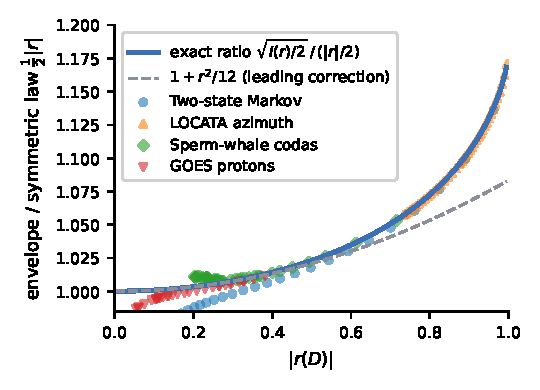
\includegraphics[width=.72\linewidth]{fig_tightness.pdf}
\caption{Tightness of the information envelope on approximately
balanced binary pairs (Proposition~\ref{prop:tight}). Curve: the exact
ratio $\sqrt{I(r)/2}\,/\,(|r|/2)$; dashes: the leading correction
$1+r^2/12$; points: per-lag plug-in ratios
$\sqrt{\hat I/2}\,/\,(|\hat r|/2)$ for the five approximately
balanced battery series ($|\hat\pi-\tfrac12|<.035$, $|r|>.05$). A
consistency illustration rather than an independent test ($\hat I$ and
$\hat r$ derive from the same pooled lag table): the plug-in points
ride the predicted curve across the full correlation range. (The ratio
to the exact \emph{value} $\widehat V_1$ lifts above this curve at
small $r$ for the mildly imbalanced series --- that is
Theorem~\ref{thm:hinge}'s threshold, not envelope slack; see
Fig.~\ref{fig:trichotomy}.)}
\label{fig:tightness}\end{figure}

Four readings, in increasing order of consequence.

\begin{figure}[t]\centering
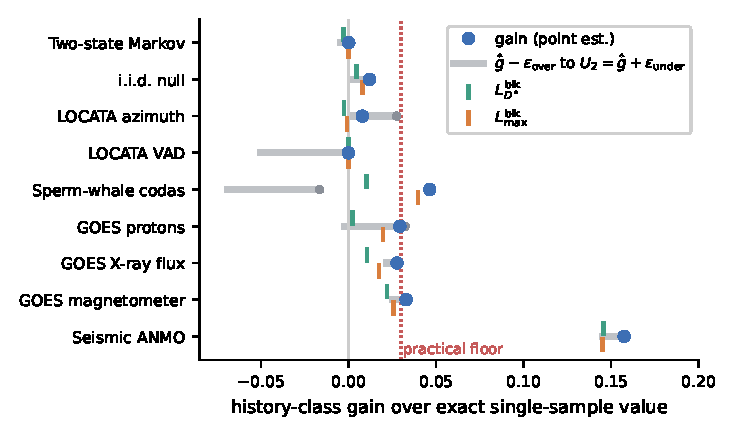
\includegraphics[width=.9\linewidth]{fig_battery.pdf}
\caption{The battery at a glance. Dots: maximum history-class gain over
the exact single-sample value; grey bars: the model-calibrated interval
$[\hat g-\varepsilon_{\mathrm{over}},\hat g+\varepsilon_{\mathrm{under}}]$;
ticks: the moving-block one-sided bounds at fixed $D^*$ (upper, teal)
and with in-replicate lag selection (lower, orange); dotted line: the
registered practical floor. Only seismic separates decisively from both
zero and the floor; the i.i.d.\ null's positive selection-aware tick
is the empirical winner's-curse floor; whale's wide bar is the
short-series noise the verdict language respects. Where
$\varepsilon_{\mathrm{under}}<0$ (whale, i.i.d.) the bias-corrected
upper endpoint $U_2$ sits \emph{below} the point estimate --- the
estimator is upward-biased there, and the bound says so.}
\label{fig:battery}\end{figure}

\textbf{The protocol corrections changed the conclusions, honestly.}
Under the original chance baseline, four series appeared to carry history
value beyond the single sample (gains $0.100$--$0.367$). Under the
majority baseline and exact $\widehat V_1$: VAD's gain vanished entirely
($+0.100\to-0.000$; $\hat\pi=.636$ --- the whole effect was the
majority-class head start), X-ray shrank $0.185\to0.028$, magnetometer
$0.147\to0.033$, and only seismic survived at strength
($0.367\to0.158$). The two-tail calibration then \emph{strengthened}
the equivalence side: $\varepsilon_{\mathrm{under}}$ is near zero or
negative on most series, so VAD and the whale codas join the
class-equivalent block. Sub-unity envelope ratios disappeared with the
imbalance correction (balanced-domain tightness ratios $1.11$--$1.35$, on
the Pinsker side of unity as population theory requires --- a consistency
illustration rather than an independent test, since $\hat I$, $\hat r$,
and $\widehat V_1$ derive from the same pooled lag table).

\textbf{Only seismic exhibits a clearly material history gain.} X-ray
and magnetometer show smaller statistically detected gains at or below
the registered practical threshold; on the remaining series \emph{no
additional value was detected by the registered six-lag lookup policy},
with class equivalence established where $U_2<0.03$ and honestly withheld
where it is not (protons, $U_2=.032$). None of these negative findings
asserts unrestricted single-sample sufficiency: a richer policy class
could in principle extract value the lookup class does not
(\S~protocol, scope of the estimand).

\textbf{An empirical dead zone.} The imbalanced GOES series exhibit
Theorem~\ref{thm:hinge}'s geometry at the plug-in level: X-ray
($\hat\pi=.421$, kink at $\tfrac12$, positive-branch threshold
$C^*\approx0.033$) has $\widehat V_1$ exactly zero across its
moderate-covariance lags --- the majority policy is unbeatable by any
single delayed sample --- while its plug-in information remains positive:
\emph{information without value}, the phenomenon of
Proposition~\ref{prop:noneq}, on a physical series. (Population
uncertainty for the dead-zone boundary itself is future work; we label
this an \emph{empirical} dead zone.)

\textbf{The conditional lower bound stands --- once at strength.} By
Theorem~\ref{thm:incr}, seismic's history gain converts into a lower
bound on conditional predictive information. The \emph{primary} result is now fully
dependence- \emph{and} selection-aware, with the correctly-stated
target: inference on the per-replicate maximum bounds the
\emph{maximal} gain over the registered lag grid, so the certificate
reads
$\max_{D\in\mathcal D} I(X_t;\text{history}_D\mid X_{t-D})
\ge 2(0.1453)^2\approx0.042$ nats --- \emph{there exists a registered
lag at which the conditional predictive information is at least
$0.042$ nats}. (A claim at the specific $D^*$ would need a simultaneous
band or sample splitting; the fixed-$D^*$ interval below is the
conditional-on-$D^*$ statement.) Two further routes
corroborate to within a few percent: the fixed-$D^*$ moving-block
interval ($[+.146,+.168]$, $\approx0.042$) and the fitted-Markov
surrogate calibration ($2(0.158-0.014)^2\approx0.041$) --- alongside the \emph{approximate} total-information witness
$I(X_t;\text{window})\gtrsim0.18$ nats (exploratory: its estimator
reuses the gain-error calibration, as noted in the protocol). History knows what the last
sample does not; that is what ``aftershock clustering'' means in
information units. Magnetometer's selection-aware bound ($+.026$, certificate
$\approx0.001$ nats) is small and reported as exploratory. The instrument reads in
both directions: class equivalence or bounded excess on most series; a
dependence-aware conditional-information lower bound exactly where the
history structure is found.

\section{Related work}\label{sec:related}

\emph{Value of information.} The Bayes envelope is the classical object of
statistical decision theory \cite{howard1966,raiffa61}, and its convex
geometry is charted territory: De Lara and Gossner \cite{delaragossner}
study the value function as a support function, characterize
\emph{exactly} when information has zero value (their Prop.~2), and prove
the small-information trichotomy our Theorem~\ref{thm:contact}
generalizes (their Prop.~10; see Remark~\ref{rem:trichotomy} for the
precise delta). Our Lipschitz lemma instantiates their payoffs--beliefs
duality; the sum-over-kinks skeleton of Theorem~\ref{thm:hinge} descends
from the mixture-of-primitives representations of statistical information
for binary experiments \cite{schervish89,reidwilliamson11}, and what is
new there is the exact lag-covariance parametrization with explicit
sign-asymmetric thresholds --- a form we have not found in that
literature, nor in the nonconcavity strand
\cite{radnerstiglitz84,chadeschlee02,delaragilotte07,whitmeyer25}; the comparison-of-experiments order behind
Lemma~\ref{lem:blackwell} is Blackwell's \cite{blackwell53}; and the
Radner--Stiglitz nonconcavity \cite{radnerstiglitz84,chadeschlee02}
anticipates the zero-marginal-value onset in smooth settings; the exact
dead zone is its polyhedral counterpart. \emph{Minimum excess risk.} The envelope inequalities of
\S\ref{sec:mi} are published results of the minimum-excess-risk
literature: the unconditional bound in \cite{makhdoumi14,gyorfi23,xu20},
the conditional form in \cite{hafezkolahi21,xuraginsky22}, the proof
engine in \cite{russo16}; Fano-type families bounding Bayes \emph{error}
by information are the classical ancestors. That literature also
contains the exact logarithmic anchor (MER under log loss \emph{equals}
conditional information; \cite{xuraginsky22}, Lem.~1), which joins the
Kelly--Barron--Cover bracket below. What we have not found there, or in
the economics of information, is the value-of-delayed-observation
framing, the inversion into certified conditional-information witnesses,
or the exact covariance-parametrized laws of \S\ref{sec:multistate}. What we have not found
elsewhere is the assembly this paper is about: the envelope \emph{anchored
to an exact law} (sharp to $O(r^3)$, with the $O(r^2)$ correction observed
on real data), its ordering against mixing envelopes with both separations
constructed, and its inversion into a certified information witness.

\emph{The logarithmic exception.} For log-utility gambling the value of
side information \emph{equals} mutual information: Kelly \cite{kelly56}
for the growth rate, Barron and Cover \cite{barroncover88} for the general
bound $\Delta\le I$ with equality characterizations. Log utility is
unbounded, escaping our $\Omega$-bounded class; the pair of results
brackets the landscape --- unbounded log utility buys equality, bounded
utility only an envelope, and Proposition~\ref{prop:noneq} shows the gap is
essential, not technical.

\emph{Age of information, and its critics.} AoI \cite{yates21} treats
freshness as the object, with sampling-policy results such as \cite{sun17}
optimizing age processes. That plain age is not decision significance is
already argued \emph{within} the field: age-of-incorrect-information
replaces the clock with an error-aware penalty \cite{maatouk20}, explicit
AoI-vs-VoI scheduling comparisons exist for networked control
\cite{ayan19}, and value-of-information metrics for feedback control have
been quantified directly, including an explicit derivation of the
value--age relation \cite{soleymani22,valueage24}. Our claim is accordingly not
that age lacks decision semantics --- that point is established --- but
sharper: for exogenous one-step bounded-reward decisions the exact semantic
object is the posterior Bayes envelope, which admits a universal
mutual-information converse, an explicit binary geometry (hinges, dead
zones, quadratic regimes), and an operational inversion into
predictive-information witnesses.

\emph{Delayed information in control.} Delayed-sharing information
structures go back to Witsenhausen \cite{witsenhausen68} and are
systematized by the common-information approach \cite{nayyar13}; remote
estimation studies the estimation face of the same trade
\cite{sun17}. Our setting is the tractable exogenous corner of that world
--- the action does not affect the state --- which is exactly what makes
closed forms and universal envelopes available.

\emph{Predictive information.} Bialek, Nemenman and Tishby
\cite{bialek01} study $I(\text{past};\text{future})$ as a measure of
process complexity. Theorems~\ref{thm:mi} and \ref{thm:hinge} are, in that
vocabulary, statements about what predictive information can and cannot buy
a bounded-utility decision maker --- with the battery's witness bound
$I\ge 2\widehat\Delta^2$ operating as a decision-theoretic estimator of
predictive information from policy value alone.

\section{Conclusion}\label{sec:conclusion}

The companion paper measured one exact law on one system. This paper
locates that law inside a unified theory of exogenous one-step
bounded-reward decisions under delay: value of delayed
information is the Bayes envelope; the envelope is bounded by predictive
information (universally), by mixing (given a model), and by the telemetry
bit rate (given nothing); for binary state it is a sign-dependent sum of hinges under polyhedral
objectives (smooth curvature giving quadratic weak-correlation response
instead), exactly a layered sum for monotone multi-state objectives, and
exactly nothing --- inside the dead zone --- for asymmetric weakly-coupled
sensing. Beyond one effective dimension, no scalar summary of dependence
determines value at all. Each claim is falsifiable, and the nine-series
battery exercises all of them: no history excess is detectable where the equivalence bound requires none,
the envelope's predicted tightness appears with its $O(r^2)$ correction,
and history gains beyond the single-sample value yield dependence-aware
lower bounds on conditional predictive information in nats. The instrument reads in both directions; that, more
than any single inequality, is what we hope survives.

\appendix
\section{Companion results restated}\label{app:companion}

For self-containedness we restate the companion results used above, with
proofs where short; \cite{infocom} is under submission and unavailable to a
reviewer.

\paragraph{Mixing coefficient.} Throughout,
$\beta(D)=\E[\sup_{B\in\mathcal F_{\ge t}}
|\mathbb P(B\mid\mathcal F_{\le t-D})-\mathbb P(B)|]$ (event-supremum
convention; a lower bound for the absolute-regularity coefficient, so the
vacuousness results transfer conservatively).

\paragraph{Binary chain.} For the symmetric two-state chain with flip
probability $p$ and $r(D)=(1-2p)^D$: conditioning on the delayed state
moves the law of $X_t$ by total variation $\tfrac12|r(D)|$ from either
value of the conditioner, and the Markov property collapses the past to the
delayed sample; hence $\beta(D)=\tfrac12|r(D)|$. The exact value of the
$0/1$ prediction objective is $\Delta(D)=\tfrac12|r(D)|$: predict the
delayed state if $r>0$, its complement if $r<0$; either beats the static
$\tfrac12$ by half the correlation magnitude.

\paragraph{Layer-cake lift (companion Prop.~2; statement and sketch).}
For capacity $a_t\in\{0,\dots,C\}$, threshold indicators
$x^u_t=\mathbf 1[a_t\ge u]$ with $\pi_u=\mathbb P(x^u_t{=}1)$, and
objectives that are positive combinations of per-layer threshold rewards
(goodput minus over-admission surplus in the companion's setting), the
objective decomposes additively over layers via
$\min(w,a)=\sum_u\mathbf 1[w\ge u]\,x^u_t$ and
$(w-a)^+=\sum_u\mathbf 1[w\ge u](1-x^u_t)$; the age-$D$ optimum applies the
per-layer binary policy (the delayed indicators, whose nesting is inherited
from the observation), and the total advantage over the best comonotone
static budget at matched surplus is
$\Delta(D)=\sum_u\pi_u r_u(D)$, $r_u(D)=\mathrm{corr}(x^u_t,x^u_{t-D})$.

\begin{thebibliography}{9}
\bibitem{infocom}
Anonymous. Companion systems submission, under review, 2026. All results
used from this reference are restated with proofs in
Appendix~\ref{app:companion}.

\bibitem{howard1966}
R.~A.~Howard. Information value theory.
\emph{IEEE Trans.\ Systems Science and Cybernetics} 2(1):22--26, 1966.

\bibitem{delaragossner}
M.~De~Lara, O.~Gossner. Payoffs-beliefs duality and the value of
information. \emph{SIAM J.\ Optimization} 30(1):287--310, 2020.

\bibitem{raiffa61}
H.~Raiffa, R.~Schlaifer. \emph{Applied Statistical Decision Theory}.
Harvard University, 1961.

\bibitem{kelly56}
J.~L.~Kelly, Jr. A new interpretation of information rate.
\emph{Bell System Technical Journal} 35:917--926, 1956.

\bibitem{barroncover88}
A.~R.~Barron, T.~M.~Cover. A bound on the financial value of information.
\emph{IEEE Trans.\ Information Theory} 34(5):1097--1100, 1988.

\bibitem{yates21}
R.~D.~Yates, Y.~Sun, D.~R.~Brown~III, S.~K.~Kaul, E.~Modiano, S.~Ulukus.
Age of information: an introduction and survey.
\emph{IEEE J.\ Selected Areas in Communications} 39(5):1183--1210, 2021.

\bibitem{sun17}
Y.~Sun, E.~Uysal-Biyikoglu, R.~D.~Yates, C.~E.~Koksal, N.~B.~Shroff.
Update or wait: how to keep your data fresh.
\emph{IEEE Trans.\ Information Theory} 63(11):7492--7508, 2017.

\bibitem{witsenhausen68}
H.~S.~Witsenhausen. A counterexample in stochastic optimum control.
\emph{SIAM J.\ Control} 6(1):131--147, 1968.

\bibitem{nayyar13}
A.~Nayyar, A.~Mahajan, D.~Teneketzis. Decentralized stochastic control with
partial history sharing: a common information approach.
\emph{IEEE Trans.\ Automatic Control} 58(7):1644--1658, 2013.

\bibitem{makhdoumi14}
A.~Makhdoumi, S.~Salamatian, N.~Fawaz, M.~M\'edard. From the information
bottleneck to the privacy funnel. In \emph{Proc.\ IEEE Information
Theory Workshop}, 501--505, 2014.

\bibitem{gyorfi23}
L.~Gy\"orfi, T.~Linder, H.~Walk. Lossless transformations and excess
risk bounds in statistical inference. \emph{Entropy} 25(10):1394, 2023.

\bibitem{xu20}
A.~Xu. Continuity of generalized entropy and statistical learning.
arXiv:2012.15829, 2020.

\bibitem{xuraginsky22}
A.~Xu, M.~Raginsky. Minimum excess risk in Bayesian learning.
\emph{IEEE Trans.\ Information Theory} 68(12), 2022.

\bibitem{hafezkolahi21}
H.~Hafez-Kolahi, B.~Moniri, S.~Kasaei, M.~Soleymani~Baghshah.
Rate-distortion analysis of minimum excess risk in Bayesian learning.
In \emph{Proc.\ ICML}, 2021.

\bibitem{russo16}
D.~Russo, B.~Van~Roy. An information-theoretic analysis of Thompson
sampling. \emph{J.\ Machine Learning Research} 17(68):1--30, 2016.

\bibitem{blackwell53}
D.~Blackwell. Equivalent comparisons of experiments.
\emph{Annals of Mathematical Statistics} 24(2):265--272, 1953.

\bibitem{radnerstiglitz84}
R.~Radner, J.~E.~Stiglitz. A nonconcavity in the value of information. In
M.~Boyer, R.~Kihlstrom (eds.), \emph{Bayesian Models in Economic Theory},
North-Holland, 33--52, 1984.

\bibitem{chadeschlee02}
H.~Chade, E.~E.~Schlee. Another look at the Radner--Stiglitz nonconcavity
in the value of information.
\emph{J.~Economic Theory} 107(2):421--452, 2002.

\bibitem{valueage24}
T.~Soleymani, J.~S.~Baras, K.~H.~Johansson. Relation between value and
age of information in feedback control. arXiv:2403.11926, 2024.

\bibitem{delaragilotte07}
M.~De~Lara, L.~Gilotte. A tight sufficient condition for
Radner--Stiglitz nonconcavity in the value of information.
\emph{J.~Economic Theory} 137(1):696--708, 2007.

\bibitem{schervish89}
M.~J.~Schervish. A general method for comparing probability assessors.
\emph{Annals of Statistics} 17(4):1856--1879, 1989.

\bibitem{reidwilliamson11}
M.~D.~Reid, R.~C.~Williamson. Information, divergence and risk for binary
experiments. \emph{J.~Machine Learning Research} 12:731--817, 2011.

\bibitem{whitmeyer25}
M.~Whitmeyer. A concavity in the value of information.
\emph{Games and Economic Behavior} 154:200--207, 2025.

\bibitem{maatouk20}
A.~Maatouk, S.~Kriouile, M.~Assaad, A.~Ephremides. The age of incorrect
information: a new performance metric for status updates.
\emph{IEEE/ACM Trans.\ Networking} 28(5):2215--2228, 2020.

\bibitem{ayan19}
O.~Ayan, M.~Vilgelm, M.~Kl\"ugel, S.~Hirche, W.~Kellerer.
Age-of-information vs.\ value-of-information scheduling for cellular
networked control systems. In \emph{Proc.\ ACM/IEEE ICCPS}, 2019.

\bibitem{soleymani22}
T.~Soleymani, J.~S.~Baras, S.~Hirche. Value of information in
feedback control: quantification.
\emph{IEEE Trans.\ Automatic Control} 67(7):3730--3737, 2022.

\bibitem{bialek01}
W.~Bialek, I.~Nemenman, N.~Tishby. Predictability, complexity, and
learning. \emph{Neural Computation} 13:2409--2463, 2001.
\end{thebibliography}


\end{document}
